\chapter{Methodology}


\section{Graph}
There are some basic properties of graphs which is important to be familiar with. Figure \ref{fig:generalGraph} depicts the basics of an unweighted graph, the edges are not assigned any value. Weighted edges can be useful to e.g. reflect capacity constraints such as a link's maximum bandwidth, or the length of a road(edge). Other common definition used when describing graphs are listed below \cite{audestad}:
\begin{itemize}
\item Edge degree: Number of edges connected with a node.
\item Hub: Node with high edge degree.
\item Cycle: A chain originating and terminating at the same node.
\item Cluster: Subgraph of highly connected nodes.
\item Cluster coefficient: Probability that two nodes that are adjacent to a third node are also adjacent.
\item Clique: Subgraph where all nodes are adjacent (cluster coefficient = 1).
\item Small world graph: Graph with small diameter and large cluster coefficient (e.g. the Internet and A-B graphs, described in section \ref{ABgraph}).
\end{itemize}

\begin{figure}[h]
\centering
\begin{tabular}{@{}c@{}}
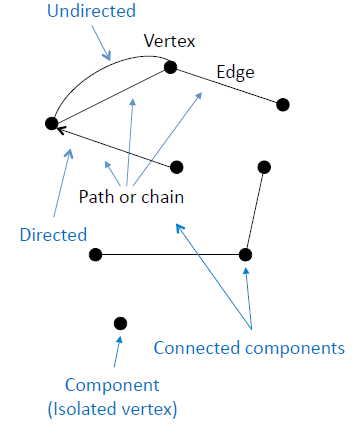
\includegraphics[width=0.4\textwidth]{../Figures/generalGraph.png}
\end{tabular}
\caption{\label{fig:generalGraph} General graph \cite{audestad}.}
\end{figure}


\section{Random Graphs}
Cyber-insurance cover many fields, from financial transactions and outsourcing of tasks to computer networks, many of these fields share a common characteristic, they can all be described as a graph, and often a random graph. Therefore the study of random graphs are of special concern. The research on random graphs are fairly new compared to other mathematical discoveries. E-R graphs were first studied in 1959 by Erdös and Rényi, later and probably with more promising results was the graphs studied by Albert-Barabási in 1999 \cite{audestad}. 
\subparagraph{Erdös-Rényi Graphs}
E-R graphs is a network created between a fixed number of $n$-nodes, where each node connects to another of the $n-1$ nodes with 
probability $p$. The resulting graph will on average contain $n(n-1)p/2 \approx n^{2}p/2$ edges \cite{barabasi}. 
By analysing the graph, the authors found some interesting properties:

\begin{itemize}
\item If $p<n^{-2}$  then there is no edges in the graph. 
\item If $p=c/n$ where c is a constant between $1 < c < log\: n$, the graph will provoke a single large component to grow within the graph.
\item If $p>(ln\: n)/n$ then the graph is completely connected. 
\item If $p = 1/n$ triangles start forming in the graph. 
\end{itemize}

A fully connected E-R graph will have a short diameter similar to the Internet, and thus could be a very good desrcription of the internet. However, the edge degree follows a Poisson distribution, which means that the edge degrees are peaking around the average value \cite{audestad}. Consequently E-R graphs does not capture the immense clustering coefficient which is present in networks such as the Internet. In other words, E-R graphs are not small world graphs, and another graph structure is needed to model computer networks.
A interesting fact about these graphs are their vulnerability, these graphs are very vulnerable against random attacks, such as nature disasters, but robust against directed attacks. Due to the fact that if you remove all edges from one node, it does little damage, since the network is not dependent on single nodes, every node has approximately the same node degree, and it is the sum of all the nodes connections that creates the network.

\subparagraph{\label{ABgraph}Albert-Barabási Graphs}
The structure which is believed to be most accurate regarding modeling computer networks are A-B graphs. A-B graphs are different from E-R graphs since they are scale-free, meaning that the vertices does not have an constant value throughout the entire graph. The formation of an A-B graph results in multiple hubs with a high edge degree. Albert and Barabási found that the edge degree of each vertex follows a power law distribution; meaning that the probability that the edge degree is $g$ is proportional to $g^{-\gamma}$
where $\gamma$ usually is a number between 2 and 3  This distribution is called a thick-tail distribution, because there is a significant probability that a node may have a very high degree. \cite{audestad}
These graphs are in contrast to E-R-graphs, very vulnerable to directed attacks, because if you take out a hub, you suddenly destroyed the whole graph. But the graph is very robust against random attacks, this is why most of the networks we observe in the nature can be depicted as A-B-graphs.
A-B graphs can grow and become scale-free if every new vertex is connected to one or more already existing node with a probability proportional to the edge degree of that node . The paper presents an algorithm that creates A-B graphs and Figure \ref{fig:ABgraphcreation} shows one graph that evolved from this algorithm:

\begin{itemize}
\item A new single vertex is added to the graph.
\item This vertex is connected to exactly two other vertices in the graph.
\item The probability that the new vertex connects to another vertex is dependent on the edge degree of the other vertex, higher edge degree meaning higher probability
\item There is only one edge between two vertices.
\end{itemize}


\begin{figure}[h]
\centering
\begin{tabular}{@{}c@{}}
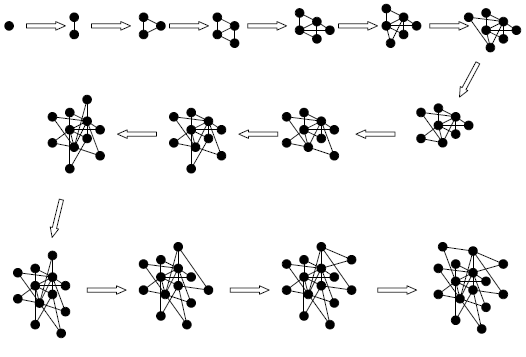
\includegraphics[width=0.8\textwidth]{../Figures/ABgraphcreation.png}
\end{tabular}
\caption{\label{fig:ABgraphcreation} Forming a A-B graph in 15 generations \cite{audestad}.}
\end{figure}

In addition to the high clustering coefficient they showed that A-B-graphs have a fairly small diameter,
 which can be seen in Figure \ref{fig:ABgraphcreation}. 
 A-B graphs are therefore comparable to the network formation of the Internet and other computer networks. 






\section{Game Theory}
Here we will present some of the game theory concepts we use in our models, for more thoroughly explanation of game theory, see: \cite{nisan2007algorithmic}.
\subparagraph{One shot game}
This type of game assumes that players act at the same time instant, therefore there is no causality. A game in strategic (normal) form can be described by three elemetns:
\begin{itemize}
\item the set of players $i \in I$, which we take to be the finite set ${1,2,....,I}$.
\item the pure-strategy space $s_{i}\in S_{i}$ for each player i, where $s_{i}$ is a possible action of player i.
\item and payoff functions $U$, which gives the players utility functions for each profile $s=(s_{1},s_{2},...,s_{I})$ of strategies.
\end{itemize}
A general solution concept for games of economic interest is the Nash Equlibrium solution. A Nash Equilibrium is a profile of strategies such that each players strategy is an best response to the other players strategies. 
\subparagraph{Nash Equilibrium}
A pure strategy profile $s^{*}$ is a Nash eqilibirum if, for all players $i$
\begin{equation}
U_{i}(s^{*}_{i},s_{-i}^{*})\geq U_{i}(s_{i},s^{*}_{-i}) \in S_{i}
\end{equation}
\subparagraph{Stackelberg}
Also known as a leader-follower game, it introduces multiple stages. The leader commits itself first, chooses its strategy, then the followers respond sequentially. The Stackelberg model can be solved to find the subgame perfect Nash Equilibrium, i.e. the strategy profile that serves each player best, given the strategies of the other players and that entails every player playing in a Nash Equilibrium in every subgame.
\subparagraph{Subgame-perfect equilibrium}
A strategy profile $s$ is a subgame perfect equilibrium if it represents a Nash Equilibrium of every subgame of the original game.
\subparagraph{Socially optimal}
A socially optimal outcome is the set of choices that maximizes the sum of all players payoffs. 
\subparagraph{Price of stability}
The price of stability (PoS) of a network game, is the ratio between the maximum sum of the players payoff, in a stable outcome, and the Socially optimal outcome.

\subparagraph{Bayesian game}
In Bayesian games, information about the other players characteristics is incomplete. In these types of games, there are one player(the agent) who knows both types, and another player (the principal) who does not know the type of the other player. 

A pooling equilibrium, is a equilibrium where all both types of the agent chooses the same action, i.e. the principal is not able to distinguish the two types. 
A separating equilibrium is an equilibrium where the agents of different types, choose different actions, and thus the principal is able to determine the agents type by observing his actions.


\section{Netlogo}
In addition to analyzing the different models with game theory, we created a simulator for the models, in a program called Netlogo. Netlogo is a programmable modeling environment for simulating natrual and social phenomena. It is well suited for modeling complex systems developing over time \cite{netlogo}.
Netlogo where good to model our complex network formation games, and at the same time provided us with a good graphical user interface, that enabled us to see the result of the games, and also to easily adjust the different parameters.
In Figure \ref{fig:netlogo} we see the user interface, which are used to setup the parameters, start the modeling, and showing the resulting network formation. Figure \ref{fig:netlogo-code} shows how the coding interface looked like. For detailed overview of the code used in our different models, see the appendix.
\begin{figure}[h]
\centering
  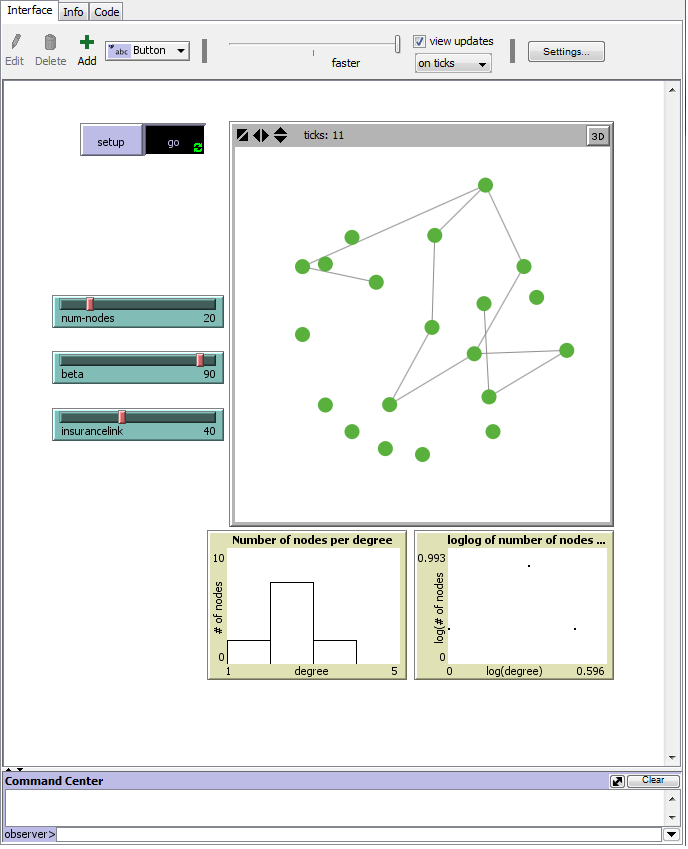
\includegraphics[width=0.9\linewidth]{../Figures/netlogoexample.png}
  \caption{\label{fig:netlogo} The figure shows a screen capture of netlogo, while we are running one of our simulations.}

\end{figure}
\begin{figure}[h]
\centering
  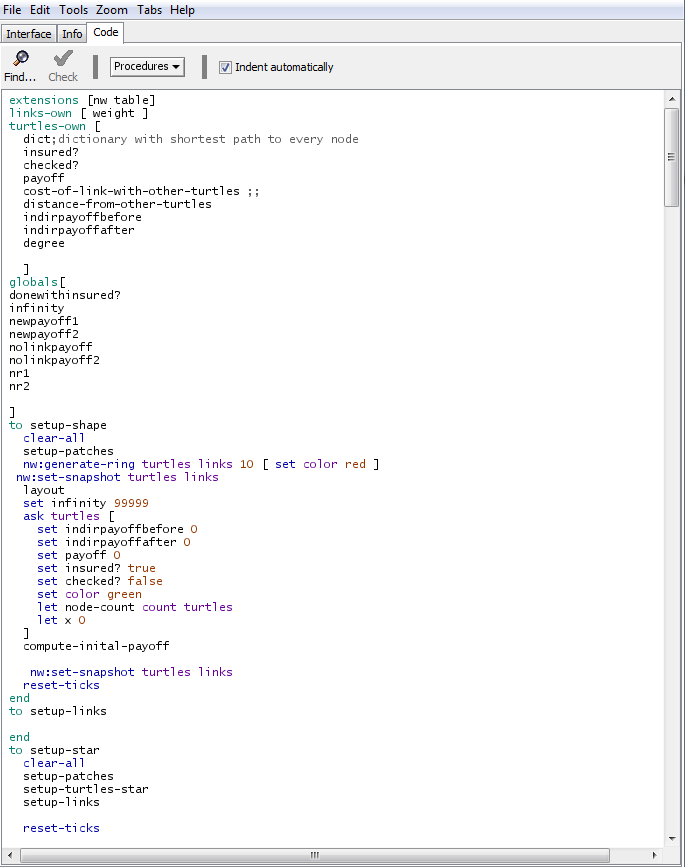
\includegraphics[width=0.9\linewidth]{../Figures/netlogocodeexample.png}
  \caption{\label{fig:netlogo-code} The figure shows how the code interface in netlogo looks like.}

\end{figure}



